\documentclass[12pt,a4paper]{article}
\usepackage{fontspec}
\usepackage{amsmath}
\usepackage{xunicode}
%\renewcommand\qedsymbol{$\blacksquare$}
\usepackage{xltxtra}
\usepackage{bbm}
\usepackage{titlesec}
\usepackage[titles]{tocloft}




\AtBeginDocument{\renewcommand\contentsname{Table of Contents}}

\titleformat{\chapter}[display]
{}{\hfill\rule{.7\textwidth}{3pt}}{0pt}
{\hspace*{.3\textwidth}\huge\bfseries}[\addvspace{-1pt}]
\titleformat{name=\chapter,numberless}[display]
{}{\hfill\rule{.7\textwidth}{3pt}}{0pt}
{\hspace*{.3\textwidth}\huge\bfseries}[\addvspace{-1pt}]
\usepackage[english,greek]{babel}

\usepackage{geometry}
 \geometry{
 a4paper,
 total={170mm,257mm},
 left=20mm,
 top=20mm,
 }
\usepackage{subfig}
\usepackage[T1]{fontenc}
\usepackage[utf8]{inputenc}
\usepackage{cancel}

\usepackage{float}

\newcommand{\lat}{\selectlanguage{english}}
\newcommand{\gre}{\selectlanguage{greek}}
\usepackage{hyperref}
\usepackage[table,xcdraw]{xcolor}
\usepackage[greek,english]{babel}
\usepackage{amsthm,thmtools}
\usepackage{amsmath}    %math
\usepackage{amsfonts}   %math fonts
\usepackage{amssymb}
\usepackage{graphicx}

\newcommand*{\tautequiv}{%
  \models\mirrormodels
}
\makeatletter
\newcommand*{\mirrormodels}{%
  \mathrel{%
    \mathpalette\reflectmathsymbol\models
  }%
}
\newcommand*{\reflectmathsymbol}[2]{%
  \reflectbox{$\m@th#1#2$}%
}
\makeatother

\usepackage{tikz}
\usetikzlibrary{matrix}
\usepackage[table]{xcolor}
\usepackage[shortlabels]{enumitem}
\usepackage{tikz,forest}
\usepackage{lmodern}

\DeclareMathOperator{\EX}{\mathbb{E}}% expected value
\usetikzlibrary{arrows.meta}

\setmainfont{CMU Serif Roman}

\newtheorem{theorem}{Θεώρημα}
\newtheorem{assumption}{Assumption}
\newtheorem{algorithm}{Algorithm}
\newtheorem{remark}{Remark}
\newtheorem{definition}{Definition}
\newtheorem{sentence}{Πρόταση}
\newtheorem{lemma}{Λήμμα}
\newtheorem{proposition}{Proposition}
\newtheorem{solution}{Λύση}
\newtheorem{note}{Σημείωση}
\declaretheoremstyle[
  headfont=\bfseries,
  bodyfont=\,
]{askhsh}

\newcommand\myeq{\mathrel{\overset{\makebox[0pt]{\mbox{\normalfont\tiny\sffamily T=1}}}{=}}}
\newcommand\myeql{\mathrel{\overset{\makebox[0pt]{\mbox{\normalfont\tiny\sffamily Fatou's Lemma}}}{\geq}}}
\newcommand\myeqd{\mathrel{\overset{\makebox[0pt]{\mbox{\normalfont\tiny\sffamily d}}}{=}}}
\newtheorem{askhsh}{Άσκηση }
\newtheorem{orismos}{Ορισμός}
\newtheorem{protash}{Πρόταση }
\newtheorem{example}{Example}
\setlength\parindent{0pt}

\newlist{SubItemList}{itemize}{1}
\setlist[SubItemList]{label={$-$}}

\let\OldItem\item
\newcommand{\SubItemStart}[1]{%
    \let\item\SubItemEnd
    \begin{SubItemList}[resume]%
        \OldItem #1%
}
\newcommand{\SubItemMiddle}[1]{%
    \OldItem #1%
}
\newcommand{\SubItemEnd}[1]{%
    \end{SubItemList}%
    \let\item\OldItem
    \item #1%
}
\newcommand*{\SubItem}[1]{%
    \let\SubItem\SubItemMiddle%
    \SubItemStart{#1}%
}%
\begin{document}

\begin{titlepage}

	\begin{center}

	\vspace{0.8cm}
	\LARGE
	NATIONAL TECHNICAL UNIVERSITY ATHENS\\
	ΚΑΝΟΝΙΣΜΟΙ ΑΓΟΡΩΝ ΕΝΕΡΓΕΙΑΣ

	\vspace{0.8cm}
	\LARGE
	SEMFE



	\end{center}
\end{titlepage}

\renewcommand{\contentsname}{Περιεχόμενα}
\tableofcontents
\pagebreak



\section{Σκοπός Εργασίας}
Σκοπός της εργασίας είναι η ανάπτυξη μεθόδων για την ταξινόμηση της ποιότητας λευκών κρασιών. Κάθε γεγονός (διαφορετικό κρασί) χαρακτηρίζεται απο 11 βιοχημικές μεταβλητές και μια βαθμολογία απο (1-10) κατόπιν γευσιγνωσίας. Το αρχείο των δεδομένων υπάρχει διαθέσιμο στο \url{https://archive.ics.uci.edu/ml/machine-learning-databases/wine-quality/winequality-white.csv}.Θεωρούμε οτι κάθε κρασί χαρακτηρίζεται ως "καλό" ή "κακό".


\begin{itemize}
\item[\cancel{a.}] Επιλέξτε το κατώφλι βαθμολογίας που διαχωρίζει τις δύο κλάσεις (π.χ μεγαλύτερη ή ίση του 5) ώστε να υπάρχει περίπου ίσος αριθμός γεγονότων κρασιών σε κάθε κλάση.
\item[\cancel{b.}] Να χωρίσετε με τυχαίο τρόπο τα δεδομένα σε σύνολο εκπαίδευσης (75\%) και σύνολο αξιολόγησης (25\%) με ίσο αριθμό γεγονότων σε κάθε κλάση.
\item[\cancel{c.}] Να απεικονίσετε για το σύνολο εκπαίδευσης τις κατανομές των 11 μεταβλητών (ένα διάγραμμα για κάθε μεταβλητή στο οποίο να φαίνεται ξεχωριστά η κατανομή για τα γεγονότα κάθε κλάσης).
\item[\cancel{d.}] Να απεικονίσετε για το σύνολο εκπαίδευσης τις συσχετίσεις όλων των μεταβλητών (ξεχωριστά για τις δύο κλάσεις).
\item[\cancel{e.}] Να κάνετε ανάλυση PCA στο σύνολο εκπαίδευσης αφού πρώτα κάνετε τυποποίηση των μεταβλητών.Δείξτε την κατανομή των ιδιοτιμών του πίνακα διασποράς.Σχολιασμός αποτελεσμάτων.
\item[\cancel{f.}] Να υλοποιήσετε έναν γραμμικό ταξινομητή ελαχιστων τετραγώνων με κατάλληλη βελτιστοποίηση των παραμέτρων του.
\item[\cancel{g.}] Να υλοποιήσετε ένα νευρικό δίκτυο (με ένα ή δύο κρυφά στρώματα και κατάλληλο αριθμό νευρώνων) που να διαχωρίζει τις δύο κλάσεις με κατάλληλη βελτιστοποίηση των παραμέτρων του.Δείξτε την καμπύλη εκπαίδευσης εκπαίδευσης και σχολιάστε το φαινόμενο της υπερεκπαίδευσης.
\item[\cancel{h.}] Να υλοποιήσετε ένα ενδυναμωμένο δέντρο απόφασης (\textbf{boosted decision tree}) που να διαχωρίζει τις δύο κλάσεις.Επιλέξτε κατάλληλο αριθμό δέντρων (μέγιστου βάθους 3).
\item[\cancel{i.}] Να συγκρίνετε την απόδοση των ταξινομητών με κατάλληλη επιλογή μετρικής και να σχολιάσετε τα αποτελεσμάτα.
\item[\cancel{j.}] Για κάθε ταξινομητή να κατατάξετε τις μεταβλητές σύμφωνα με την επίδραση τους σε αυτόν (backwards selection).Σχολιάστε τις ομοιότητες και διαφορές μεταξύ  των διαφορετικών ταξινομητών.



\end{itemize}


\newpage
\section{Report - White wine classification}

Σκοπός της εργασίας που μας δόθηκε είναι η ταξινόμηση της ποιότητας λευκών κρασιών.Κάθε γεγονός αντιπροσωπεύει ένα διαφορετικό κρασί το οποίο χαρακτηρίζεται απο 11 διαφορετικές βιοχημικές μεταβλητές:
\begin{itemize}
\item Alcohol : Ποσότητα αλκοόλης (\%).
\item Sulphates: Ποσότητα θειικών αλάτων στο κρασί (g/dm3).
\item pH : pH του κρασιού (κλίμακα 0-14).
\item density (g/dm3).
\item total sulfurdioxide : Ποσότητα SO2 στο κρασί.
\item free sulfurdioxide : Ελεύθερη μορφή SO2 (mg/dm3)
\item chlorides : Ποσότητα Χολωριούχου νατρίου (αλατιού) (g/dm3).
\item residual sugar : Ποσότητα ζάχαρης μετά την ζύμωση (g/dm3).
\item volatile acifity : Ποσότητα οξικού οξέος στο κρασί (g/dm3)
\item fixed acidity : Ποσότητα τρυγικού οξέος (g/dm3)
\item citric acid : Ποσότητα κιτρικού οξέος (g/dm3)
\end{itemize}
Κάθε μια απο τις επεξηγηματικές μεταβλητές είναι ποσοτική.Στην συνέχεια η ποιότητα του κρασιού περιγράφεται μέσω μιας κλίμακας απο (1-10).Όσο υψηλότερη είναι η τιμή της μεταβλητής quality τόσο καλύτερη είναι και η ποιότητα του κρασιού.Σκοπός μας είναι να ταξινομήσουμε τα λευκά κρασία που μας δίνονται σύμφωνα με τις βιοχημικές μεταβλητές και την αξιολόγηση σε \textbf{"καλό"} ή \textbf{"κακό"}.To σύνολο των παρατηρήσεων είναι 4899 λευκά κρασιά.

\par
\subsection{Προπαρασκεύη των Δεδομένων}
Αρχικά βρίσκουμε το κατώφλι βαθμολογίας το οποίο διαχωρίζει τις δύο κλάσεις (\textbf{"καλό"} , \textbf{"κακό"}) με σκοπό να έχουμε περίπου τον ίδιο αριθμό παρατηρήσεων στις δύο κλάσεις.Σχεδιάζουμε λοιπόν ένα ιστόγραμμα για να παρατηρήσουμε την κατανομή των βαθμολογιών που δόθηκαν στην κλίμακα (0-10).Το διάγραμμα παρουσιάζεται παρακάτω.

\begin{figure}[H]
\centering
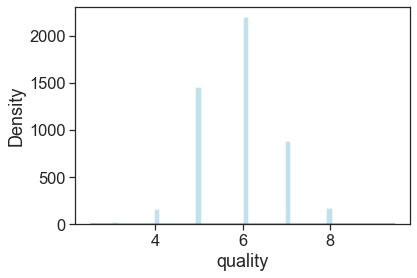
\includegraphics[width=0.30\linewidth,height=0.20\textheight]{Images/plot1}
\caption{Histogram for quality}
\label{fig:imagea}
\end{figure}
Μπορούμε λοιπόν εύκολα να παρατηρήσουμε οτι μια λογική τιμή που θα μπορούσε να διαχωρίσει την ποιότητα του κρασιού σε δύο κλάσεις είναι κοντά στο ($ \approx $ 6.5).Δηλαδή θεωρούμε οτι όσα κρασιά έχουν αξιολόγηση μεγαλύτερη του 6.5 είναι \textbf{"καλά"} ενώ τα υπόλοιπα αξιολογούνται ως \textbf{"κακά"}.Τελικά έχουμε 3838 παρατηρήσεις για τα κρασιά με βαθμολογία κάτω του οριού αξιολόγησης και 1060 παρατηρήσεις για αυτά πάνω απο το όριο αξιολόγησης.

\begin{figure}[H]
\centering
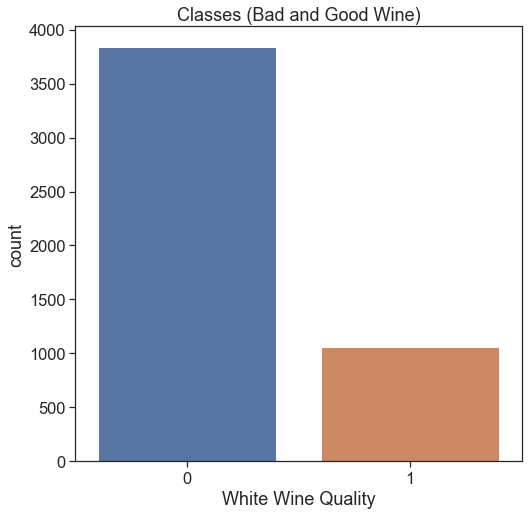
\includegraphics[width=0.30\linewidth,height=0.20\textheight]{Images/plot2}
\caption{Classes for White Wine quality}
\label{fig:imagea}
\end{figure}



\par Στην συνέχεια χωρίζουμε τα δεδομένα σε σύνολο εκπαίδευσης και σύνολο αξιολόγησης με τυχαίο τρόπο.Σύμφωνα με τα δεδομένα της εργασίας ο διαχωρισμός γίνεται σε ένα σύνολο εκπαίδευσης (75 \%) των συνολικών παρατηρήσεων και σύνολο αξιολόγησης (25\%) με ίσο αριθμό γεγονότων σε κάθε κλάση.Μπορούμε να δούμε οτι στο αρχικό σύνολο δεδομένων η κατανομή ανάμεσα στις δύο κλάσεις δεν είναι σταθερή.Εμείς θέλουμε όμως τα σύνολα εκπαίδευσης και αξιολόγησης να έχουν τον ίδιο αριθμό παρατηρήσεων σε κάθε κλάση.Για να το επιτύχουμε αυτό αρχικά χωρίζουμε με τυχαίο τρόπο το αρχικό μας σύνολο και στην συνέχεια με τυχαίο τρόπο για καθένα απο τα σύνολα εκπαίδευσης και αξιολόγησης διαγράφουμε τις τιμές της κλάσης εκείνης που έχει τον μεγαλύτερο αριθμό παρατηρήσεων.Τελικά καταλήγουμε με
\begin{itemize}
\item Σύνολο Εκπαίδευσης : 1576 Παρατηρήσεις
\item Σύνολο Αξιολόγησης : 544 Παρατηρήσεις
\end{itemize}
\begin{figure}[H]
    \centering
    \subfloat[\centering Before Undersampling]{{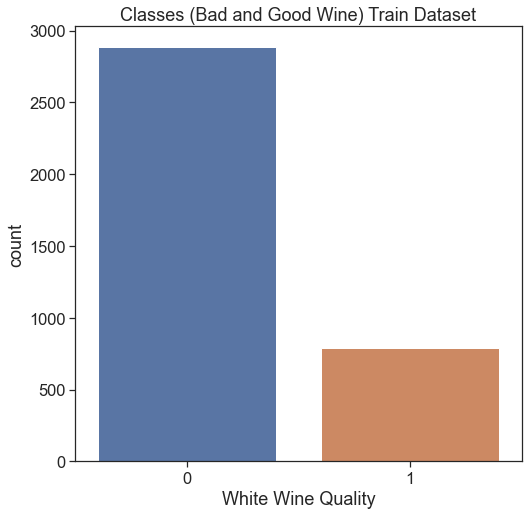
\includegraphics[width=5cm]{Images/plot3} }}%
    \qquad
    \subfloat[\centering Balanced Dataset]{{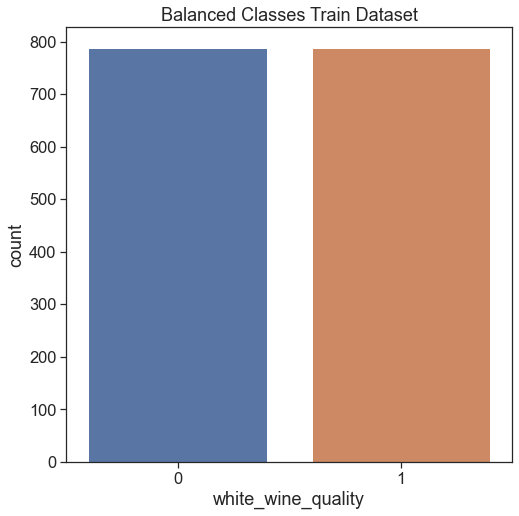
\includegraphics[width=5cm]{Images/plot4} }}%
    \caption{Balance Train Dataset}%
    \label{fig:example}%
\end{figure}

\newpage
Με όμοιο τρόπο για το σύνολο αξιολόγησης έχουμε
\begin{figure}[H]
    \centering
    \subfloat[\centering Before Undersampling]{{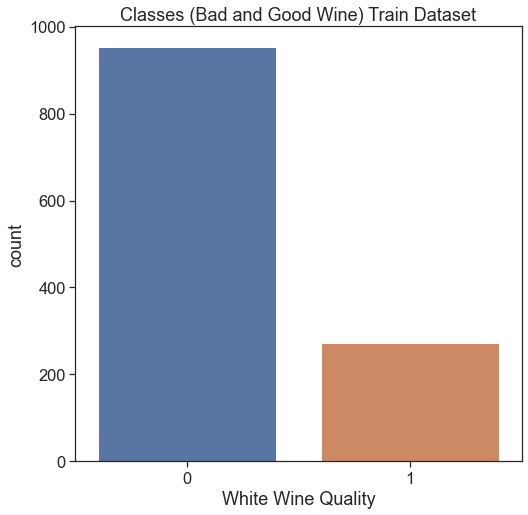
\includegraphics[width=5cm]{Images/plot5} }}%
    \qquad
    \subfloat[\centering Balanced Dataset]{{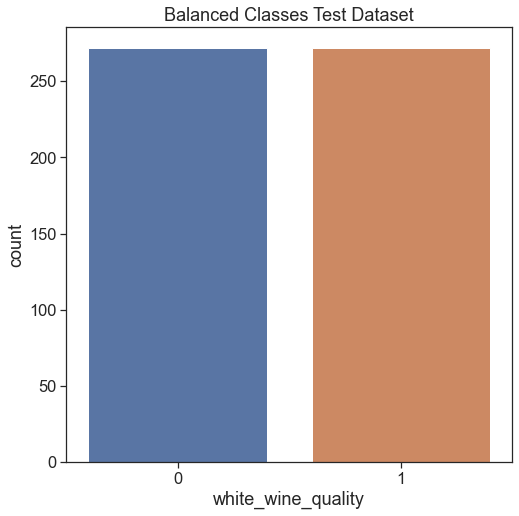
\includegraphics[width=5cm]{Images/plot6} }}%
    \caption{Balance Test Dataset}%
    \label{fig:example}%
\end{figure}

Έχοντας ολοκληρώσει τον διαχωρισμό των δεομένων μας στα δύο υποσύνολα συνεχίζουμε εξετάζοντας τις κατανομές των επεξηγηματικών μεταβλητών σε κάθε ένα απο τα σύνολα ξεχωριστά.Αρχικά για το \textbf{σύνολο εκπαίδευσης} παρατηρούμε παρακάτω τις κατανομές των μεταβλητών καθώς και την μεταξύ τους εξάρτηση.

\begin{figure}[H]
\centering
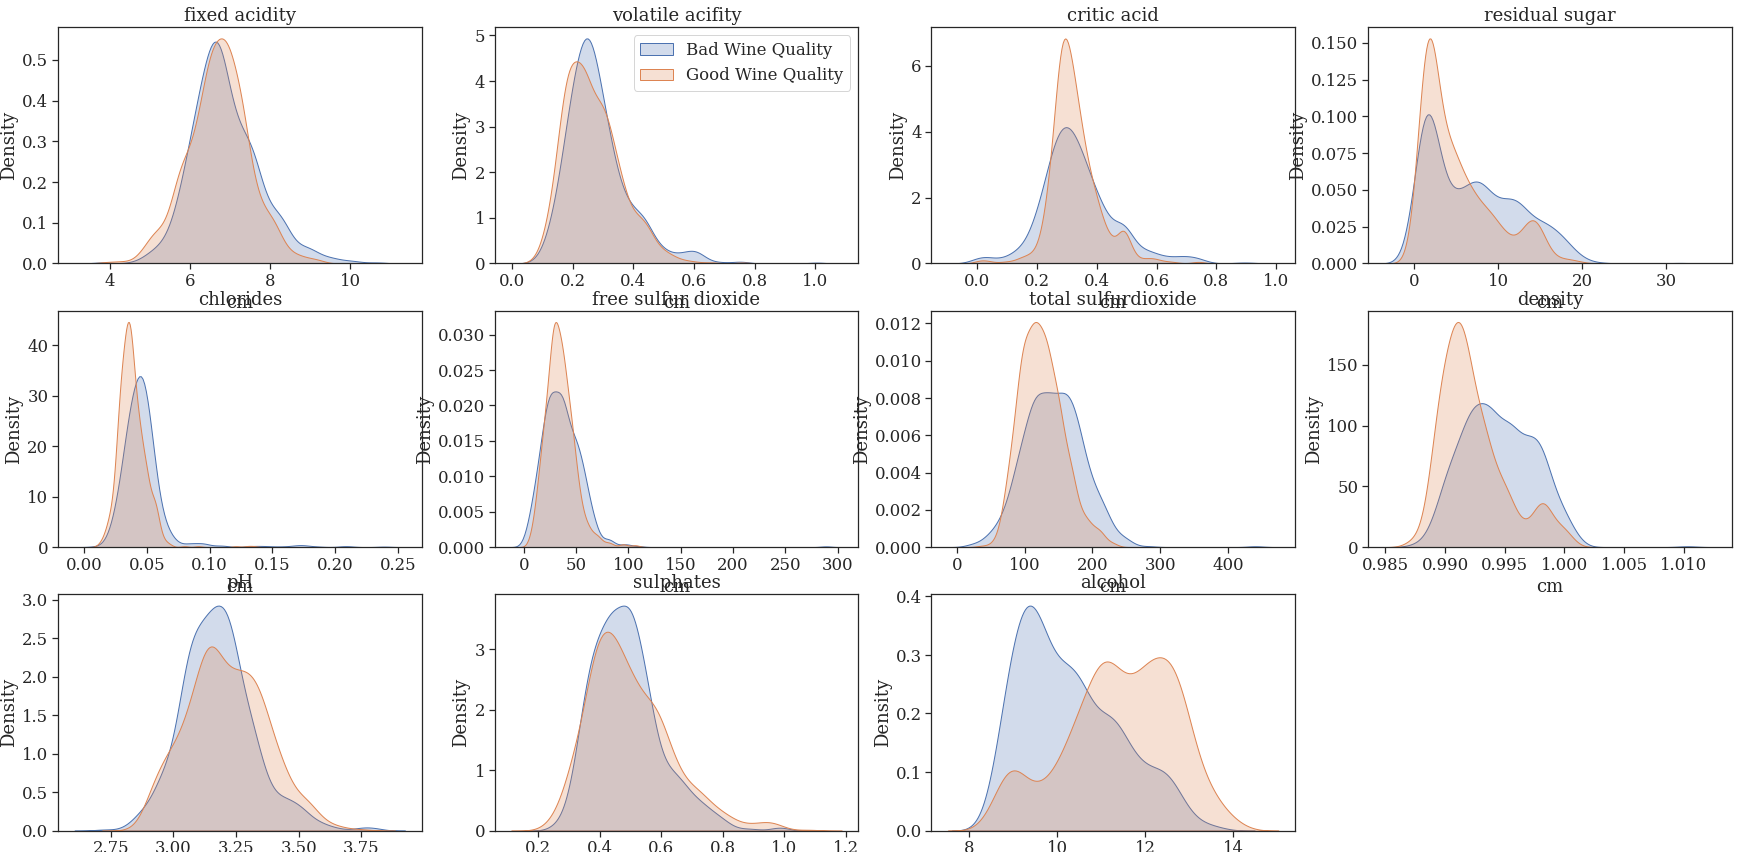
\includegraphics[width=0.70\linewidth,height=0.50\textheight]{Images/plot7}
\caption{Distribution of Variables}
\label{fig:imagea}
\end{figure}


Μπορούμε να συμπεράνουμε οτι οι μεταβλητές που φαίνεται να έχουν υψηλό βαθμό διαχωρισιμότητας είναι οι \textbf{Density , Alcohol}.



\par Έπειτα κατασκευάζουμε τα διαγράμματα των πινάκων συνδιασποράς για το σύνολο εκπαίδευσης και για καθεμια απο τις διαφορετικές κλάσεις (\textbf{"καλό"} , \textbf{"κακό"} κρασί) για να ελέγξουμε αν υπάρχουν εμφανείς διαφορές σχετικά με την συσχέτιση των μεταβλητών ανάμεσα στις δύο κλάσεις.


\begin{figure}[H]
    \centering
    \subfloat[\centering Correlation for Good Wines Class]{{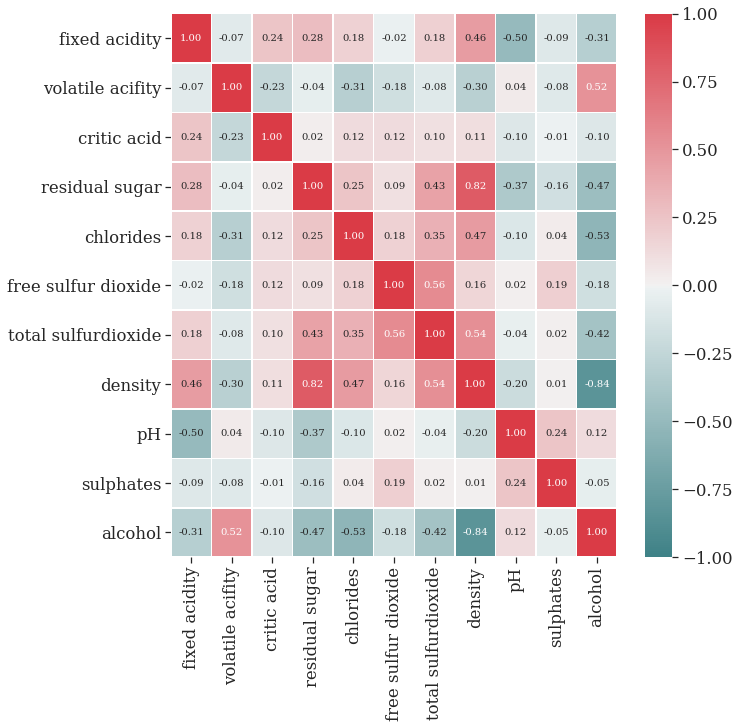
\includegraphics[width=9cm,height=6cm]{Images/plot9} }}%
    \qquad
    \subfloat[\centering Correlation for Bad Wines Class]{{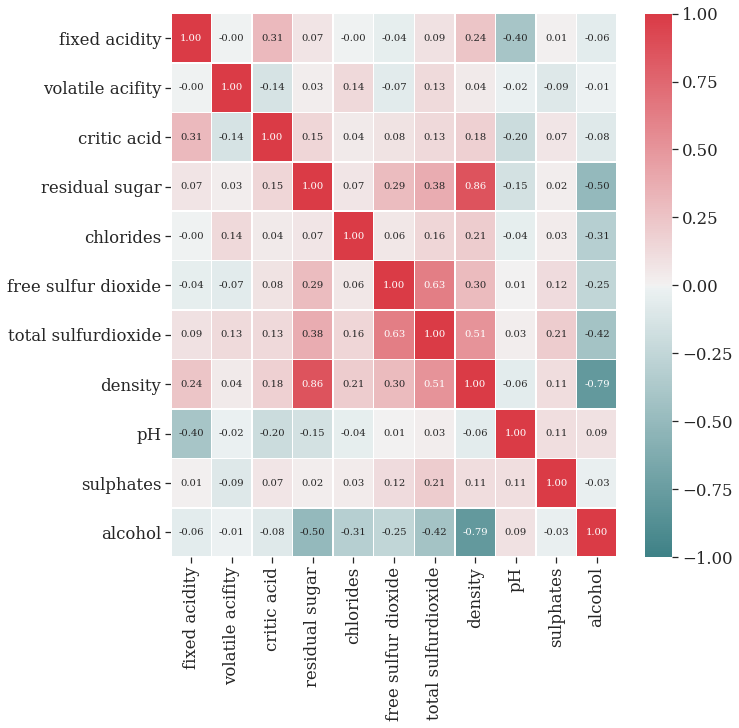
\includegraphics[width=9cm,height=6cm]{Images/plot10} }}%
    \caption{Correlations Train Dataset}%
    \label{fig:example}%
\end{figure}

Απο το παραπάνω διάγραμμα μπορούμε να παρατηρήσουμε μια σημαντική διαφορά μεταξύ της συσχέτισης των μεταβλητών (\textbf{volatile acidity} - \textbf{Alcohol}).Συγκεκριμένα στο σύνολο εκπαίδευσης για την κλάση κρασιών με αξιολόγηση <6.5 παρατηρούμε οτι οι δύο μεταβλητές είναι ασυσχέτιστεσ.Σε αντίθεση με την κλάση καλών κρασιών όπου η συσχέτιση των δύο μεταβλητών είναι θετική ($ \approx$ 0.5).Δεν φαίνεται να υπάρχουν αλλές διαφορές που μπορούν να παρατηρηθούν απο το παραπάνω διάγραμμα συνεπώς συνεχίζουμε με τεχνικές μείωσης χαρακτηριστικών του προβλήματος.

\subsection{Variable Reduction Techniques}
Θα ξεκινήσουμε την ανάλυση μας με μια απο τις πιο γνωστές μεθόδους μείωσης διαστάσεων την (PCA - Principal Component Analysis).Η ιδέα να δημιουργήσουμε ένα hyperplane το οποίο βρίσκεται όσο πιο κοντά γίνεται στα δεδομένα και στην συνέχεια να προβάλουμε τα δεδομένα μας σε αυτο.Σκοπός μας είναι να εξετάσουμε ποιές μεταβλητές έχουν μεγαλύτερη διαφορά ανάμεσα στις δύο κλάσεις και επίσης ποιές απο αυτές περιγράφουν το μεγαλύτερο μέρος της διασποράς του δείγματος.Ο αλγόριθμος βρίσκει τους άξονες που περιγράφουν το μεγαλύτερο μέρος της διασποράς του δείγματος και μας επιστρέφει ένα μικρότερο υποσύνολο των διαστάσεων που περιγράφουν την διασπορά των δεδομένων.Ο αλγοριθμος περιγράφεται παρακάτω:
\begin{itemize}
\item Αρχικά τυποποιούμε τα δεδομένα
$$z = \frac{x-\mu}{\sigma} \ \  where  \ \ \mu = \frac{1}{N}\sum_{i=1}^N (X_i)$$
and $$\sigma = \sqrt{\frac{1}{N}\sum_{i=1}^N(X_i -\mu)^2 } $$
\item Στην συνέχεια υπολογίζουμε τον πίνακα διασποράς
$$Cov = \frac{1}{n-1} \sum_{i=1}^n (X_i-\bar{x})(Y_i - \bar{y})$$
\item Βρίσκουμε τις ιδιοτιμές και τα ιδιοδιανύσματα του $X^TX$.
\item Κατατάσοπυμε τις ιδιοτιμές σε φθίνουσα σειρά και ο πίνακας στήλη είναι ο $P^*$ (θετικά ορισμένος)
\item Βρίσουμε τις νέες τιμές
$$Z^* = ZP^*$$
όπου ο νέος αυτός πίνακας περιέχει τις τυποποιημένες X και έχουμε προβάλει τις τιμές στον νέο χώρο διάστασης.



\end{itemize}

Τελικά μπορούμε να κατασκευάσουμε ένα διάγραμμα για την κατανομή των ιδιοτιμών στον πίνακα συνδιασποράς.Το αποτέλεσμα είναι το ακόλουθο.
\begin{figure}[H]
    \centering
    \subfloat[\centering Eigenvalues Distribution]{{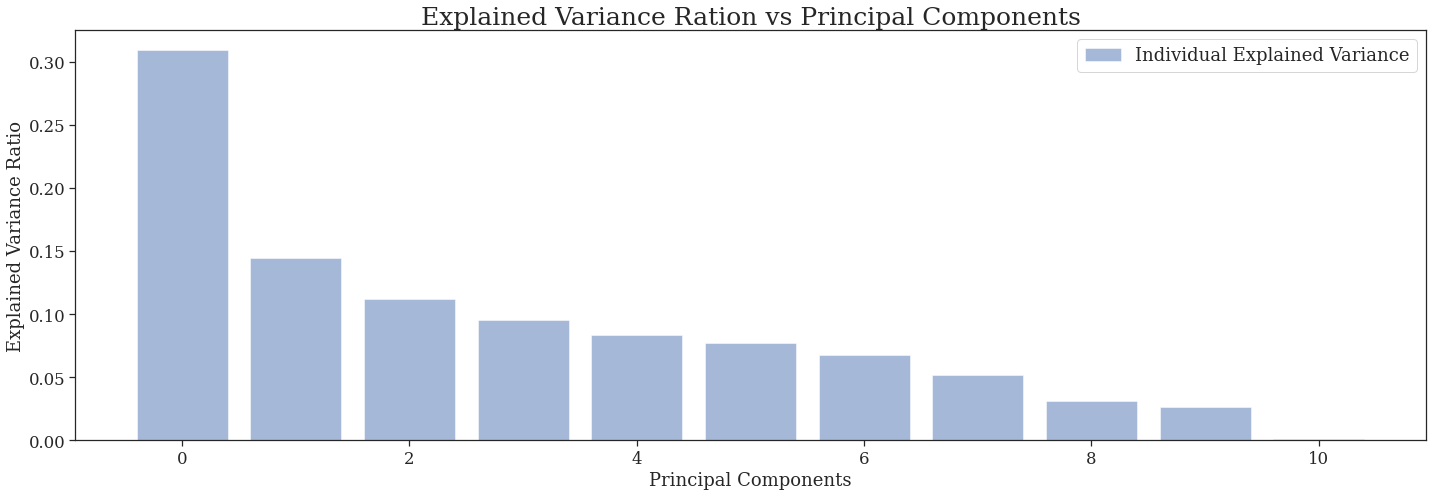
\includegraphics[width=7cm,height=4cm]{Images/plot11} }}%
    \qquad
    \subfloat[\centering Explained Variance]{{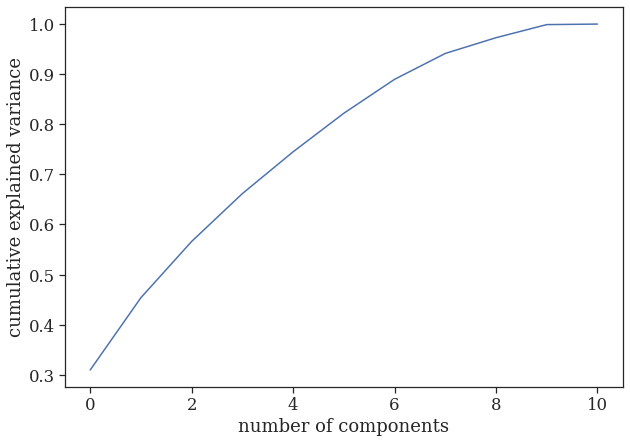
\includegraphics[width=7cm,height=4cm]{Images/plot12} }}%
    \caption{PCA plots}%
    \label{fig:example}%
\end{figure}
Μπορούμε να παρατηρήσουμε απο τα παραπάνω διαγράμματα οτι σχεδόν ($\approx$ 90\%) της διασποράς του δείγματος περιγράφεται απο τα πρώτα 6 Principal Components.Μπορούμε λοιπόν στην ανάλυση των ταξινομητών που θα παρουστεί στα επόμενα κεφάλαια να διαλέξουμε τις 6 κύριες συνιστώσες ώστε να μειώσουμε και την πολυπλοκότητα των αλγορίθμων (The Curse of Dimensionality).
\newpage
\subsection{Μοντέλα Ταξινόμησης}
\subsubsection{Linear discriminant analysis -Γραμμικός Ταξινομητής}
Θα συνεχίσουμε την ανάλυση μας σχετικά με την μείωση διαστάσεων χρησιμοποιώντας έναν γραμμικό ταξινομητή ελαχίστων τετραγώνων.Συγκεκριμένα αν θεωρήσουμε ενα σύνολο $\Sigma = \{x_1,x_2,..,x_N\}$ ένα σύνολο εκπαίδευσης με $x_i = (x_{i1} , ...,x_{id})$ και $y(x_i)$ το επιθυμητό αποτέλεσμα ταξινόμησης δύο κλάσεων (π.χ $ y_i=1 $ για x$\in \omega_1$ και $y_i=0$ για $x\in \omega_2$).Θα κατασκευάσουμε έναν γραμμικό ταξινομητή που \textbf{ελαχιστοποιεί} το συνολικό σφάλμα.Η μετρική (συνάρτηση κόστους) που θα διαλέξουμε είναι
$$J(w) =\sum_{i=1}^N(\underbrace{y_i}_{real \ value} - \underbrace{x_i^Tw}_{prediction})^2$$
Σκοπός μας είναι να ελαχιστοποιήσουμε την συνάρτηση κόστους
$$\frac{\partial J}{\partial w} = 0 $$
το οποίο μας δίνει
$$\sum_{i=1}^N (x_i (y_i-x_i^T\hat{w})) =0 \implies \hat{w} = (X^TX)^{-1}(X^TY)$$
Τα προβλήματα που μπορούν να προκύψουν στην μέθοδο ελαχίστων τετραγώνων είναι
\begin{itemize}
\item Μεγάλος όγκος δεδομένων (πολυπλοκότητα).
\item Ο πίνακας ($X^TX$) μπορεί να μην είναι αντιστρέψιμος.
\end{itemize}
Ένα ακόμη πρόβλημα για τους ταξινομητές LDA είναι οτι έχουν ως βασική προυπόθεση
$$P(X|y=k) =\frac{1}{(2\pi)^{d/2}|\Sigma_k|^{1/2}}exp(-\frac{1}{2}(X- \mu_k)^t \Sigma_k^{-1}(X-\mu_k))$$
Δηλαδή  οι δεσμευμεένες πιθανότητες ακολουθούν κανονική κατανομή.

\newpage

\subsubsection{Νευρωνικό Δίκτυο}
Ο \textbf{Perceptron} είναι μια απο τις απλούστερες αρχιτεκτονικές νευρωνικού δικτύου , η οποία ανακαλύφθηκε απο τον Frank Rosenblatt το 1957.Eίναι βασισμένος σε ένα νευρώνα ο οποίος καλείται threshold logic unit (TLU).Οι είσοδοι και έξοδοι είναι αριθμοί και κάθε είσοδος είναι συνδεμένη με τις υπόλοιπες μέσω ενός βάρους.O TLU υπολογίζει λοιπόν ένα αρθοισμά με βάρη
$$z = w_1x_2 + w_2x_2 + ... w_nx_n = X^TW$$
και ύστερα μέσω μίας βηματικής συνάρτησης (step function) μας δίνει το αποτέλεσμα (output).
$$h_w(x) = step(z)$$

\begin{figure}[H]
\centering
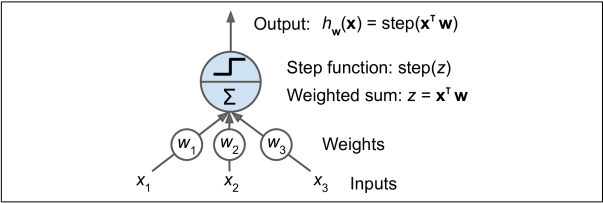
\includegraphics[width=0.60\linewidth,height=0.20\textheight]{Images/plot14}
\caption{TLU Architecture}
\label{fig:imagea}
\end{figure}

Μερικές απο τις πιο γνωστές βηματικές συναρτήσεις είναι η συνάρτηση \textbf{Heaviside} ή sgn(z)
$$heaviside(z) =\begin{cases}
0 \ z<0 \\
1 \ z\geq 0\\
\end{cases} \ \ \ \\ sgn(z) =\begin{cases}
-1 \ \ z<0\\
0 \ \ z=0\\
1 \ \ z>0\\
\end{cases}$$
Παρακάτω θα εξετάσουμε περισσότερες συναρτήσεις ενεργοποιήσης που χρησιμοποιούνται στην αρχιτεκτονική νευρωνικών δικτύων.

\par Όπως είδαμε ένας Perceptron απλά αποτελείται απο ένα μόνο στρώμα TLU το οποίο συνδέεται με όλα τα στρώματα εισόδου.Η αρχιτεκτονική αυτή όμως καθιστά αδύνατον για το Perceptron να λύσει προβήματα όπως (Exclusive OR (XOR) classification) το οποίο ισχύει για κάθε μοντέλο γραμμικού ταξινομητή όπως π.χ Logistic Regression Classifiers.Ωστόσο, πολλούς απο αυτούς τους περιορισμούς μπορούμε να τους λύσουμε χρησιμοποιώντας πολλαπλά Perceptrons.Το ANN που παράγεται με τον τρόπο αυτό είναι γνωστό ως Multilayer Perceptron (MLP).

\par Η αρχιτεκτονική ενός Multilayer Perceptron αποτελείται απο ένα \textbf{στρώμα εισόδου (input layers)} , ένα ή περισσότερα στρώματα TLU τα οποία ονομάζουμε \textbf{κρυφά στρώματα (hidden layers)} και ένα τελευταίο στρώμα TLU (\textbf{στρώμα εξόδου (output layer)}).

\begin{figure}[H]
\centering
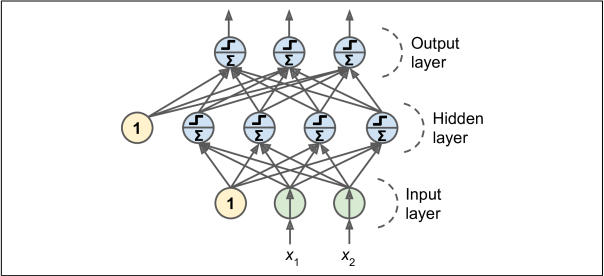
\includegraphics[width=0.60\linewidth,height=0.20\textheight]{Images/plot15}
\caption{Multilayer Perceptron Architecture}
\label{fig:multi}
\end{figure}

\begin{note}
  \end{note}


Παρατηρούμε οτι το ANN που περιγράφεται στην παραπάνω εικόνα έχει κατεύθυνση μόνο προς την μεριά της εξόδου.Η αρχιτεκτονική αυτή είναι ένα παράδειγμα \textbf{feedforward neural network (FNN)}.


\subsubsection{Εκπαίδευση Νευρωνικού Δικτύου}
Αρχικά θα ασχοληθούμε με το forward propagation (ή forward pass).Η διαδικασία αυτή είναι η διαδικασία κατά την οποία γίνεται ο υπολογισμός και η αποθηκευση των παραμέτρων του ANN μαζί με τις μεταβλητές εξόδου (input layer $\to$ output layer).Θα θεωρήσουμε λοιπόν οτι έχουμε ένα $x \in R^d$ διάνυσμα εισόδου  τότε μπορούμε να γράψουμε την αναλυτική μορφή ενός ANN με την ακόλουθη αρχιτεκτονική \ref{fig:multi}.H έξοδος του jth κρυφού στρώματος μπορεί να υπολογιστεί έναν γραμμικό συνδυνασμό με βάρη για τις d τιμές εισόδου και προσθέτοντας τα αντοίστοιχα bias.

$$a_j = \sum_{i=1}^d w_{ji}^(1)x_i + w_{j0}(1) \ \ \ (A)$$
όπου  $ w_{ji}^(1) $ δηλώνει ένα βάρος για το πρώτο στρώμα , απο την είσδο (i) μέχρι το κρυφό στρώμα (j) και $ w_{j0}(1)$ to bias για το κρυφό στρώμα j.Στο συγκεκριμένο ANN μπορούμε να δοούμε οτι η τιμή του bias είναι σταθερά 1.Για να ''ενεργοποιήσουμε'' λοιπόν το κρυφό στρώμα j μετασχηματίζουμε το γραμμικό άρθροισμα (A) χρησιμοποιώντας μις συνάρτηση ενεργοποίησης όπως αναφέραμε
$$z_j =g(a_j)$$
Συνεχίζουμε την διαδικασία αφού οι έξοδοι τροφοδοτούνται στο επόμενο στρώμα.Συνεπώς για κάθε έξοδο k δημιουργούμε τον γραμμικό συνδυνασμό των εξόδων και έχουμε
$$a_k = \sum_{j=1}^M w_{kj}^{(2)}z_j + w_{k0}^{(2)}$$
Τέλος η ενεργοποίηση της k εξόδου υπολογίζεται μετασχητίζοντας τον γραμμικό συνδυασμό μέσω μιας \textbf{μη γραμμικής} συνάρτησης και λαμβάνουμε
$$y_k =\tilde{g(a_k)}$$
\begin{note}

\end{note}
Ο λόγος που χρησιμοποιούμε διαφορετική συνάρτηση για το στρώμα εξόδου είναι για να δηλώσουμε οτι δεν χρειάζεται να είναι ίδια συνάρτηση με τα κρυφά στρώματα.

Μπορούμε να συνδυάσουμε τα παραπάνω και να καταληξουμε στην ακόλουθη επαναληπτική διαδικασία
$$y_k = \tilde{g}(\sum_{j=0}^M w_{kj}^{(2)}g(\sum_{i=0}^d w_{ji}^{(1)x_i}))$$


\textbf{Συναρτήσεις Ενεργοποίησης}

\begin{itemize}
\item Βηματικές Συναρτήσεις (Step Functions) : Χρησιμοποιούνται όπως είδαμε παραπάνω στον ορισμό του Perceptron
$$g(x) =
\begin{cases}
1  \ \ x \geq x>= 0.5\\
0 \ \ else\\
  \end{cases}$$

\item Σιγμοειδής Συνάρτησεις (Sigmoid Activation) : Είναι απο τις πιο γνωστές οικογένεις συναρτήσεων για τα feedforward neural networks και η έξοδος μέσω αυτου του μετασχηματιμού δίνει αποκλειστικά θετικές τιμές.H συνάρτηση sigmoid  είναι :
$$g(x) =\frac{1}{1 + e^{-x}}$$
\item Υπερβολική Εφαπτομένη (Hyperbolic Tangent) : Επίσης ανήκει στην οικογένεια των Σιγμοιειδών συναρτήσεων αλλά με τιμές -1 και 1.
$$g(x)=tanh(x)$$
\item ReLU (Rectified Linear Unit) : Μια απο τις πιο γνωστές συναρτήσεις στην χρήση τους για τα feedforward NN , καθώς προσφέρει γρήγορους υπολογισμούς.
$$g(x) =max(0,x)$$
όπου x η είσοδος του νευρώνα.
\item Softmax Activation Function : Χρησιμοποιείται στο στρώμα εξόδου και είναι πολύ χρήσιμη σε προβλήματα ταξινόμησης.Η έξοδος δεν είναι μια τιμή αλλά η πιθανότητα μια παρατήρηση να ανήκει στις κλάσεις του προβλήματος ταξινόμησης.Είναι απαραίτητο οι πιθανότητες να αρθοίζουν στην μονάδα.Για να πάρουμε την πιθανότητα χρησιμοποιούμε την softmax συνάρτητη με τον ακόλουθο τρόπο
$$g_i(x) = \frac{e^{z_i}}{\sum_{j\in Group}e^{z_j}}$$
όπου j αντιπροσωπεύει όλους τους νευρώνες στην κλάση.H μεταβλητή z ορίζει τις εξόδους του νευρώνων.


\end{itemize}




\begin{figure}[H]
\centering
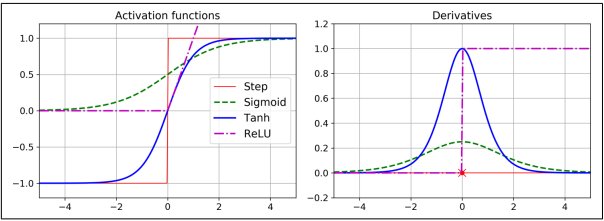
\includegraphics[width=0.60\linewidth,height=0.20\textheight]{Images/plot16}
\caption{Multilayer Perceptron Architecture}
\label{fig:multi}
\end{figure}


\textbf{Συνάρτηση Κόστους - Cost Function}


\par Μια σημαντική παράμετροσ για τον σχεδιασμό ANN είναι η επιλογή της συνάρτησης κόστου.Εφόσον έχουμε υπολογίσει τις εξόδους του NN σκοπός μας είναι να υπολογίσουμε την συνάρτηση κόστους και να την ελαχιστοποιήσουμε.Ορισμένες απο τις πιο γνωστές συναρτήσεις κόστους είναι
\begin{itemize}
  \item MSE (Mean squared error)  :
  $$MSE = \frac{1}{n} \sum_{i=1}^n (y_i-\hat{y_i})^2$$
 Παρουσιάζει προβλήματα σε περίπτωση ακραίων τιμών.
\item MAE (Mean Absolute error) :
$$MAE = \frac{1}{n}\sum_{i=1}^n |y_i - \underbrace{\hat{y_i}}_{pred}| $$

\item Huber Cost Function :
$$L(X,Y;\theta ,t_H) =
\begin{cases}
\frac{1}{2} \sum_{i=0}^{N-1}(y_i-\hat{y_i})^2 \ \ \ |(y_i-\hat{y_i})| \leq t_H\\
t_H \sum_{i=0}^{N-1}|y_i-\hat{y_i}| - \frac{t_H}{2} \ \ \ |(y_i-\hat{y_i})| > t_H\\
  \end{cases}$$
όπου $t_H$ ένα επίπεδο αναφοράς τέτοιο ώστε για αποστάσεις μικρότερες του $t_H$ να έχουμε τετραγωνικές τιμές για την συνάρτηση κόστους ενώ για αποστάσεις $> t_H$ μετασχηματίζουμε σε γραμμική συνάρτηση.Με τον τρόπο αυτό μειώνουμε την επίδραση του σφάλματος για τυχούσες ακραίες τιμές.


 \item Binary Cross Entropy :
 $$J(X) =-\sum_{i=1}^N P(x_i) log q(x_i) = -\frac{1}{N} \sum_{i=1}^N y_i \cdot log(p(y_i)+(1-y_i)log(1-p(y_i)))$$
 όπου y η ετικέτα κάθε κλασής και $p(y)$ η πιθανότητα να ανήκει στην κλάση 0.Χρησιμοποιείται σε προβλήματα ταξινόμησης.
\end{itemize}

Ωστόσο η εκπαίδευση ενός ANN μέσω forward propagation δεν είναι πάντα εύκολη.Στο να ξεπεραστεί αυτό το πρόβλημα σηματνικό ρόλο κατέχει ο αλγόρθμος \textbf{back propagation} , κατα τον οποίο υπολογίζουμε τα βάρη ενός ANN κατά την εκπαίδευση με αντίστροφη διαδικασία απο το στρώμα εξόδου στο στρώμα εισόδου.O τρόπος με τον οποίο δουλεύει είναι υπολογίζοντας την μεταβολή των βαρών ($ v_t$) για κάθε βάρος ($\theta$) στο NN.Αφαιρώντας λοιπόν την διαφορά αυτή απο κάθε βάρος έχουμε μια εκτίμηση της μορφής
$$\theta_t =\theta_{t-1} -v_t$$
Η μεταβολή αυτή τώρα εξαρτάται απο τον αλγόριθμο που διαλέγουμε.Κλασσικοί αλγόριθμοι back propagation απλώς υπολογίζουν την κλιση (gradient ($\nabla$)) για κάθε βάρος στο NN σε συνδυασμό με το \textbf{cost function} που περιγράψαμε παραπάνω.Η κλίση πολλαπλασιάζεται με έναν συντελεστή εκμάθησης.
$$v_t = \eta \nabla_{\theta_{t-1}}J(\theta_{t-1})\ \ \ (B)$$

Μπορούμε εύκολα λοιπόν να δούμε οτι το back propagation που περιγράδουμε στην (B) είναι μια μορφή Μεθόδου	απότομης	καθόδου(gradient descent method).

\newpage

Περιγράφουμε λοιπόν τα βήματα που ακολουθεί ο αλγόριθμος Back propagation και συγκεκριμένα με ο αλγόριθμος Gradient descent.
\begin{itemize}
\item Χρησιμοποιείται ένα mini-batch την φορά , και ελέγχει ολόκληρο το σύνολο εκπαίδευσης πολλαπλές φορές.Κάθε επανάληψη ονομάζεται \textbf{epoch}.
\item Στην συνέχεια κάθε mini-batch περνάει απο το στρώμα εισόδου του ANN το οποίο με την σειρά του το στέλνει στο πρώτο κρυφό στρώμα.Ο αλγόριθμος υπολογίζει την έξοδο όλων των νευρώνων σε αυτό το στρώμα.Η ίδια διαδικασία συνεχίζει για όλα τα κρυφά στρώματα της αρχιτεκτονικής μέχρι να φτάσουμε στο στρώμα εξόδου.Αυτή η μέθοδος έχει συζητηθεί ήδη παραπάνω κια είναι γνωστή ως \textbf{forward propagation}.
\item Στην συνέχεια ο αλγόριθμος υπολογίζει το σφάλα εξόδου , δηλαδή χρησιμοποεί μια συνάρτηση κόστους όπως συζητήσαμε παραπάνω και συγκρίνει τις προβλέψεις με τα πραγματικά αποτελέσματα και επιστρέφει ένα μέτρο που περιγράφει το σφάλμα.
\item Έπειτα υπολογίζει "πόσο" επηρεάζει κάθε σύνδεση εξόδου στο σφάλμα.Αυτό επιτυγχάνεται χρησιμοποιώντας τον κανόνα αλυσίδας.

\item Ο αλγόριθμος μετράει ύστερα πόσο απο αυτό το σφάλμα προήλθε απο την σύνδεση με τον προηγούμενο στρώμα , δουλεύοντας προς τα πίσω μέχρι να φτάσει στο στρώμα εισόδου.Αυτή η διαδικασία ουσιαστικά υπολογίζει την κλίση του σφάλματος σε όλα τα συνδεδεμένα βάρη.
\item Τέλος ο αλγόριθμος χρησιμοποιεί την μέθοδο απότομης καθόδου (Gradient descent method)
$$w(t+1) = w(t) - \rho_t \nabla_w J \ \ \  (1)$$
για να μεταβάλει όλα τα βάρη στο NN χρησιμοποιώντας το σφάλμα που έχει ήδη υπολογίσει.
\end{itemize}

Μπορούμε εύκολα να δούμε οτι για τον παραπάνω αλγόριθμο Gradient descent , αν θεώρήσουμε οτι έχουμε μια κυρτή συνάρτηση κόστους τότε χρησιμοποιώντας Taylor Expansion μπορούμε να γράψουμε οτι $$J \approx J(w^*) + \frac{1}{2}\frac{\partial^2 J }{\partial w^2}(w - w^*)^2$$
Συνεπώς στην επαναληπτική διαδικασία (1) έχουμε οτι
$$w(t+1) = w(t) -\rho \frac{\partial J}{\partial w} = w(t) - \rho \frac{\partial ^2 J}{\partial w^2}(w(t) - w^*)$$
$$\rho_0 = (\frac{\partial^2 J}{\partial w^2})^{-1}$$

Υπάρχουν αρκετοί ακόμη αλγόριθμοι που σκοπεύουν στην βελτιστοποίηση του ΑΝΝ.Ορισμένοι απο τους πιο δημοφιλείς είναι
\begin{itemize}
\item Adagrad
\item Adam
\item Momentum
\item RMSProp
\item SGD(Stochastic Gradient descent)
\end{itemize}

Θα κάνουμε μια γρήγορη αναφορά στον αλγόριθμο Adam (το οποίο είναι ένα απο το πιο cited papers στον τομέα του AI) και έχει πάρει το όνομα του απο την διαδικασία που χρησιμοποιεί (adaptive moment estimates).Ο αλγόρθμος Adam υπολογίζει τις πρώτες δύο ροπές (μέση τιμή , διασπορά) για να υπολογίσει τα βάρη διόρθωσης.O Adam ξεκινάει με μια εκθετικά φθίνουσα μέση τιμή για τα gradients
$$\mu_t = \beta_1 \mu_{t-1} +(1-\beta_1)\underbrace{g_t}_{current  \ \ gradient}$$
Στην συνέχεια υπολογίζει την ίδια επαναληπτική διαδικασία για τη δευτερη ροπή
$$v_t = \beta_2 v_{t-1} + (1-\beta_2) g_t^2$$
όπου τώρα οι $m_t , v_t$ είναι εκτημήτριες των πρώτων δυο ροπών της κλίσης.Το bias για την πρώτη ροπή διορθώνεται ως
$$\hat{m_t} = \frac{m_t}{1-\beta_1^t}$$
και για την δεύτερη ροπή
$$\hat{v_t} = \frac{v_t}{1-\beta_2^t}$$
Τελικά έχουμε για την επαναληπτική διαδικασία του αλγοτιθμου Adam οτι
$$\theta_t = \theta_{t-1} -\frac{a\hat{\mu_t}}{\sqrt{\hat{v_t}} +\eta}\hat{\mu_t}$$
Ο αλγόριθμος Adam είναι πολυ ευαίσθητος ώς προς την αλλαγή των παραμέτρων του.Οι Kingma και Ba (2014) προτείνουν τιμές $\beta_1 =0.9 \ \ \beta_2=0.999 \ \  \eta=10^{-8} $


\par {\textbf{Προβλήματα Εκπαίδευσης/Βελτιστοποίσης Νευρωνικών Δικτυών}}

\par Γνωρίζουμε οτι ακόμη και η κυρτή βελτιστοποίηση είναι ένα δύσκολο κομμάτι των Μαθηματικών.Σε περιπτώσει μάλιστα που δεν έχουμε συναρτήσεις κόστους οι οποίες είναι κυρτές τα πράγματα είναι ακόμη πιο περίπλοκα.Μερικά απο τα προβλήματα που μπορεί να συναντήσουμε είναι
\begin{itemize}
\item Ill Conditioning (Αναφερόμαστε στα προβήματα που μικρές μεταβολές στις αρχικές συνθήκες μπορούν να επηρεάσουν αισθητά το τελικό αποτέλεσμα): Κατά την εκπαίδευση του NN και όταν χρησιμοποιείται ο αλγόριθμος SGD μπορεί η εκπαίδευση να "κολήσει"
\item .....

\end{itemize}











\newpage
\par \textbf{Σημασία Ρυθμού εκμάθησης}

\begin{figure}[H]
    \centering
    \subfloat[\centering Optimal Learning Rate]{{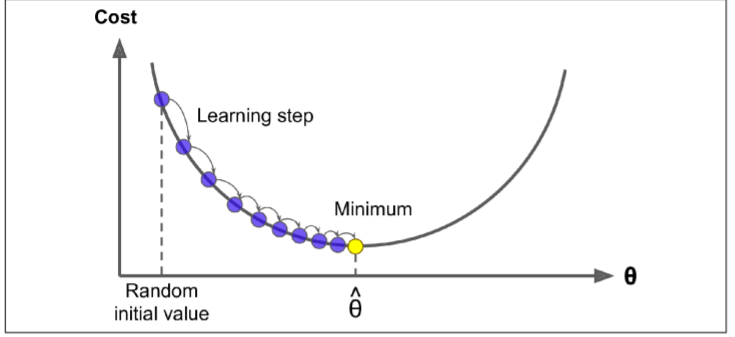
\includegraphics[width=5cm,height=4cm]{Images/plot18} }}%
    \qquad
    \subfloat[\centering Small Learning Rate]{{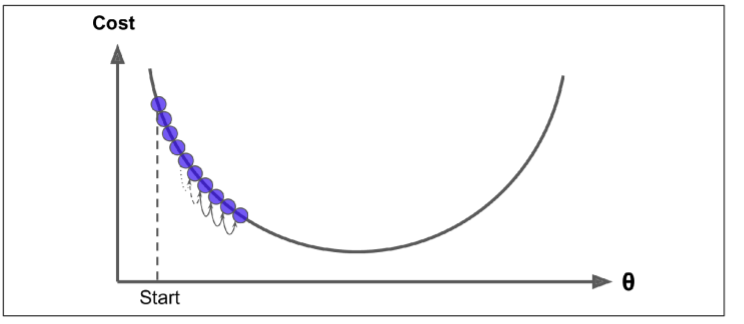
\includegraphics[width=5cm,height=4cm]{Images/plot19} }}%
    \qquad
    \subfloat[\centering Large Learning Rate]{{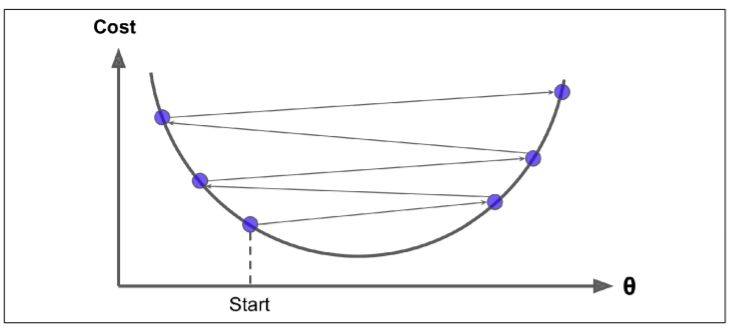
\includegraphics[width=5cm,height=4cm]{Images/plot20} }}%
    \caption{Example for Convex Cost Function -Learning Rate}%
    \label{fig:example}%
\end{figure}




\subsection{Decision Trees}
Τα δέντρα αποφάσεων είναι αλγόριθμοι μηχανικής μάθησης , που μπορούν να χρησιμοποιήθούν και σε προβλήματα ταξινόμησης καθώς και σε προβλήματα παλινδρόμησης.Ο τρόπος με τον οποίο λειτουργούν τα \textbf{Decision Trees} είναι οτι λαμβάνουν μια σειρά αποφάσεων ή κανόνων η οποίες συνήθως εξαρτώνται απο μια παράμετρο ανά φορά.Αυτός ο διαχωρισμός του δέντρου χωρίζει την είσοδο (δειγματικό χώρο) σε περιοχές που χαρακτηρίζουν την ακρίβεια σε κάθε επίπεδο μέχρι να καταλήξουμε στο βάθος (τερματισμό) του δέντρου όπου περιέχει και την τλεική πρόβλεψη.Ένα δέντρο απόφασης περιέχει τα ακόλουθα χαρακτηριστικά
\begin{itemize}
\item Node (Διαχωρισμός) : Είναι το σημείο όπου γίνεται ο διαχωρισμός στα τρμήματα και λαμβάνεται μια απόφαση.

\item Root Note (Πρώτος Διαχωρισμος)
\item Branches : Το βέλος που περιέχει την σύνδεση ενός των Node

\item Leaf Node : Το τελικό Node του δέντρου

\end{itemize}

Έχοντας λοιπόν κάνει τους διαχωρισμούς χρειαζόμαστε έναν συστηματικό τρόπο να υπολογίζουμε την "πληροφορία".


Ένα δέντρο απόφασης είναι ένας μηχανισμός πρόβλεψης $h : X \to Y$ ο οποίος προβλέπει την ταμπέλα μιςα παρατήρησης x , μέσω μιας διαδικασίας προσπέλασης ενός δέντρου απο την αρχή μέχρι ένα leaf.Για ευκολία θα αναφερθούμε σε ένα binary classification πρόβλημα , όπως αυτό που μας έχει δοθεί.


\begin{figure}[H]
\centering
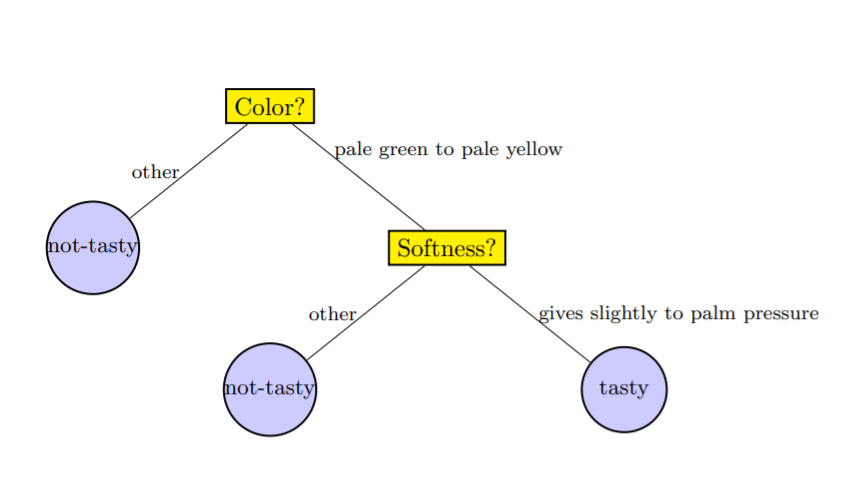
\includegraphics[width=0.40\linewidth,height=0.30\textheight]{Images/plot21}
\caption{Understanding Machine Learning,
 2014 by Shai Shalev-Shwartz and Shai Ben-David
Published 2014 by Cambridge University Press}
\label{fig:multi}
\end{figure}

Ένας βασικός τρόπος για να δημιουργούμε ένα δέντρο απόφασης είναι να ξεκινήσουμε με ένα δέντρο που έχει μόνο ένα leaf (root) και να θέσουμε σε αυτό μια ετικέτα σύμφωνα με την πλειοψηφία  των ψηφων ανάμεσα σε όλες τις ετικές του συνόλου εκπαίδευσης.Στην συνέχεια ακολουθούμε μια επαναληπτιή διαδικασία.Σε κάθε επανάληψη μελετάμε την επίδραση ενός διαχωρισμού.Ορίζουμε μια μετρική "πληροφορίας" που μετράει κατά ποσο υπάρχει βελτίωση λόγο του διαχωρισμού.Αν΄λαμεσα σε όλους τους πιθανούς διαχωρισμού , διαλέγουμε εκίνον που μεγιστοποιεί το gain(μετρική) που έχουμε ορίσει.Υπάρχουν πολύ αλγόριθμοι που είναι μορφής δέντρου.Μερικοί απο τους πιο γνωστούς είναι
\begin{itemize}
\item ID3 (Iterative Dichotomizer 3)
\item CART
\item C.45
\end{itemize}


\begin{figure}[H]
\centering
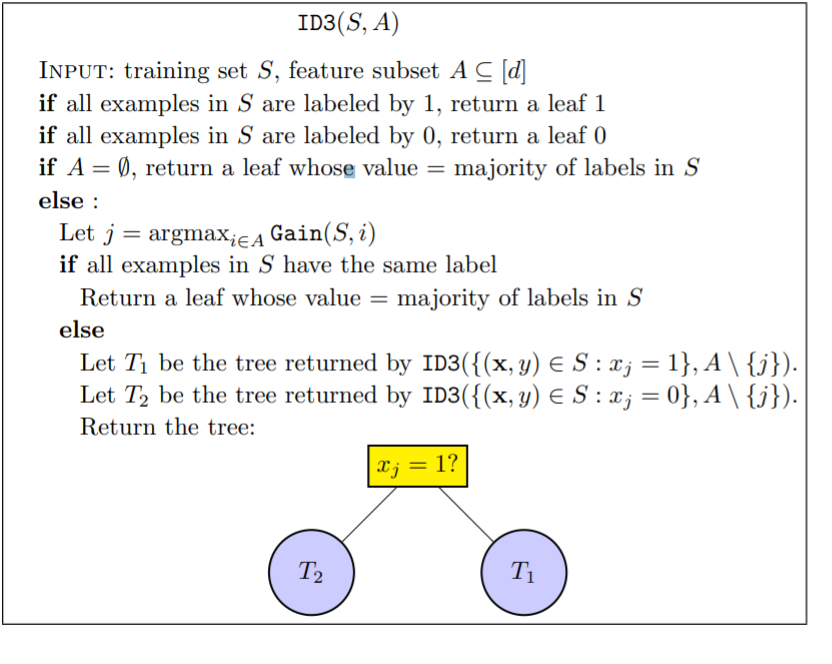
\includegraphics[width=0.40\linewidth,height=0.30\textheight]{Images/plot22}
\caption{ ID3 Algorithm - Understanding Machine Learning,
 2014 by Shai Shalev-Shwartz and Shai Ben-David
Published 2014 by Cambridge University Press}
\label{fig:multi}
\end{figure}

Στο παραπάνω περιγράδουμε τον αλγόριθμο ID3.Στο σημείο που εμφανίζεται η συνάρτηση Gain(S,i) πρέπει να αναφέρουμε οτι υπάρχουν πολλά διαφορετικά μέτρα που χαρακτηρίζουν το "gain":

\begin{itemize}
\item Information gain :Η έννοια της πληροφορίας θα οριστεί ως
$$\textbf{"Information" \ \ from \ \ observing  \ \  event   \ \ occurence}=$$
$$ \# bits \ \ encoding\ \ propability \ \ of p = -log_2p$$

Αν λοιπόν θεωρ΄λησουμε οτι έχουμε πολλαπλά ενδεχόμενα , ποια είναι η μέση πληροφορια αυτών;
\par Έστω λοιπόν οτι τα σενάρια αυτά $v_1,..,v_j$  έχουν πιθανότητα εμφάνισης
$p_1,..,p_J$ με [$p_1,..,p_J$].Τότε
$$\mathbb{E}_{p\sim[p_1,..,p_j]} I(p) = -\sum_jp_j log_2 p_j = H(p)$$
ονομάζουμε H(p) entropy της διακριτής κατανομής.
\par Αν λοιπόν έχουμε 2 ενδεχόμενα με πιθανότητα p= [p,1-p] τότε
$$H(p) = -plog_2(p) - (1-p)log_2 (1-p)$$

\item Gini Index : Χρησιμοποιείται απο τον αλγόριθμο CART $$I(a) = 2a(1-a)$$



\item Train error : Η μείωση του σφάλματος εκπαίδευσης επίσης είναι ένα λογικό μέτρο για να μετράει το "gain".Έστω I - min\{a,1-a\}.Πρίν γίνει ο διαχωρισμός στο χαρακτηριστικό i έχουμε οτι $C(P_s[y=1])$ όπου $P_s[F]$ είναι η πιθανότητα ένα ενδοχόμενο να ισχύει κάτω απο την ομοιόμορφη κατανομή.Μετά λοιπόν τον διαχωρισμό στο i έχουμε οτι $$P_S[x_i=1]C(P_S[y=1|x_i=1])+P_S[x_i=0]C(P_S[y=1|x_i=0])$$

άρα το gain μπορούμε να το ορίσουμε ως
$$Gain(S,i) = C(P_s[y=1]) -P_S[x_i=1]C(P_S[y=1|x_i=1])+P_S[x_i=0]C(P_S[y=1|x_i=0]) $$
\end{itemize}





\subsection{Boosted Decision Trees}

Η διαδικασία Boosting είναι μια ισχυρή τεχνική η οποία συνδυάζει πολλαπλά μοντέλα ταξινόμησης για να φτίαξει ένα μοντέλο με καλυτερη απόδοση.Ένα απο τα πιο γνωστά μοντέλα είναι το AdaBoost το οποίο μελετήθηκε απο τους Freund και Schapire (1996).H βασική διαφορά τη μεθόδου Boosting απο αυτήν του bagging είναι οτι κάθε base ταξινομητής εκπαιδεύτεται σε σειρά  (sequentially), και επίσης κάθε base ταξινομητής εκπαιδεύεται χρησιμοποιώντας τα δεδομένα μαζί με ένα βάρος το οποίο προέρχεται απο την απόδοση του πρηγούμενου σε σειρά ταξινομητή.Όταν τελικά ο ταξινομητής έχει εκπαιδευτεί οι προβλέψεις συνδυάζονται παίρνοντας το βεβαρυμένο μέσο όρο όλων των base ταξινομητών.

\par Ας θεωρήσυμε λοιπόν ένα πρόβλημα ταξινόμησης δύο κλάσεων όπου τον σύνολο εκπαίδευσης αποτελείται απο ένα δυάνυσμα $x_1,..x_N$ χαρακτηριστικών και μια binary μεταβλητή απόκρισης $t_1,...,t_N$ με $t_n \in \{-1,1\}$.Σε κάθε  δεδομένο δίνεται ένα βάτος $w_n$.Θέλουμε να κατασκευάσουμε έναν άλλον ταξινομητή $f(x) = sign(F(X))$
με
$$F(x) = \sum_k a_k \phi(x;w_k)$$
Δηλαδή εκπαιδεύουμε με τα ίδια δεδομένα πολλούς ταξινομητές και κατόπιν παίρνουμε το άρθροισμα τους με βάρη $a_k$ (διαφορεικά βάρη).



\begin{figure}[H]
\centering
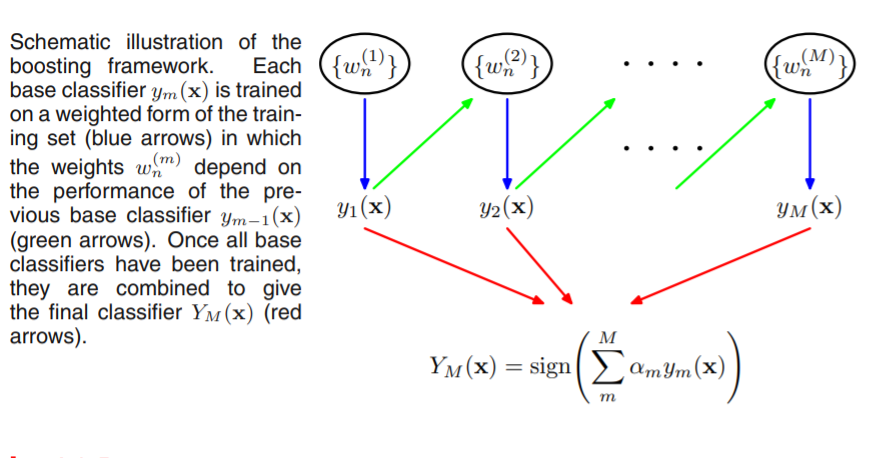
\includegraphics[width=0.90\linewidth,height=0.30\textheight]{Images/plot23}
\caption{boosting - Understanding Machine Learning,
 2014 by Shai Shalev-Shwartz and Shai Ben-David
Published 2014 by Cambridge University Press}
\label{fig:multi}
\end{figure}

\textbf{Περιγραφή Ααλγορίθμου AdaBoost}
\begin{itemize}
\item Αρχικοποιούμε τα βάρη $\{w_n\}$  ως $\{w_n^{(1)}\} =1/N $
\item Για m=1,...,M
\begin{itemize}
\item[a.] Κάνουμε fit εναν ταξινομητή $y_m(x) $ στο σύνολο εκπαίδευσης ελαχιστοποιώντας την συνάρτηση σφάλματος
$$J_m = \sum_{n=1}^N w_n^{(m)} \mathbbm{1}(y_m(x_n) \neq t_n)$$
\item[b.] Υπολογίζουμε τις ποσότητες
$$\epsilon_m = \frac{sum_{n=1}^N w_n^{(m)} \mathbbm{1}(y_m(x_n) \neq t_n)}{\sum_{n=1}^Nw_n}$$
και βρίσκουμε
$$a_m = ln\{\frac{1-\epsilon_m}{\epsilon_m}\}$$
\item[c.] Ανανεώνουμε τα βάρη των δεδμένων
$$w_n^{(m+1)} = w_n^mexp\{a_m\mathbbm{1}(y_m(x_n) \neq t_n)\} $$

\end{itemize}
\item Κάνουμε πρόβλεψη χρησιμοποι'ώντας το τελικό μοντέλο
$$Y_M(x) = sign(\sum_{m=1}^M a_m y_m(x))$$


\end{itemize}


Ένας ακόμη πολύ γνωστός αλγόριθμος Boosting είναι ο \textbf{Gradient Boosting} , ο οποίος αρχικά δημοσιεύθηκε το 1997 στο paper του Leo Breiman's "Arching the Edge"  , και στην συνέχεια μελετήθηκε απο τον Jerome H.Friedman το 1999.Ο τρόπος με τον οποίο λειτουργεί ο αλγόριθμος αυτός είναι αρκετά κοντά με τον AdaBoost , δηλαδή διαδοχικά προσθέτει τα βάρη για τα μοντέλα που εκπαιδεύει διορθώνοντας αυτά που ακολουθούν.Η διαφορά είναι οτι εδώ αντί να διορθώνει τα βάρη σε κάθε βήμα όπως ο AdaBoost , η μέθοδος αυτή προσπαθεί να κάνει fit το νέο μοντέλο πρόβλεψης στα υπόλοιπα που προκύπτουν απο το προηγούμενο μοντέλο.

\par \textbf{Αλγόριθμος Gradient Boosting}

Έστω ένα σύνολο εκπαίδευσης $\{x_i , y_i \}_{i=1}^n$ και μια συνάρτηση κόστους $\in C^1$ $L(y,F(x))$ , και ένας αριθμός επαναλήψεων M
\begin{itemize}
\item[1.] Αρχικοποιούμε το μοντέλο με μια σταθερά $$F_0 = argmin_{\gamma} \sum_{i=1}^n L(y_i, \gamma)$$

\item[2.] Για m=1 μέχρι M
\begin{itemize}
\item[a.] Υπολογίζουμε τα "ψεύτικα" σφάλματα
$$r_{im} = -[\frac{\partial L(y_i,F(x_i))}{\partial F(x_i}]$$
\item[b.] Κάνουμε fit έναν αρχικό δέντρο και το εκπαιδεύουμε χρησιμοποιώντας τα $\{(x_i, r_{im})_{i=1}^n\}$
\item[c.] Βρίσκουμε έναν πολλαπλασιαστή λύνοντας το πρόβλημα βελτιστοποιήσης
$$\gamma_m = argmin_{\gamma} \sum_{i=1}^n L(y_i,F_{m-1}(x_i) +\gamma h_m(x_i))$$
\item[d.] Κάνουμε την επαναληπτική διαδικασία
$$F_m(x) = F_{m-1}(x) +\underbrace{v}_{learning \ Rate}\cdot\gamma_x h_m(x)$$
\item[3.] Έξοδος του μοντέλου $F_M(x)$.


\end{itemize}


\end{itemize}



\newpage



\subsection{Performance Measures - Μετρικές απόδοσης}

Έχοντας περιγράψει παραπάνω ορισμένους απο τους βασικούς αλγορίθμους μηχανικής μάθησης για ταξινόμησης καθώς και την χρήση των ANN θα αναφέρουμε παρακάτω τις μετρικές με τις οποίες θα αξιολογήσουμε την απόδοση των μοντέλων που κατασκευάσαμε.Η αξιολόγηση ενός ταξινομητή δεν είναι τόσο εύκολη διαδικασία καθώς υπάρχει πληθώρα μετρικών απο τις οποίες μπορούμε να επιλέξουμε.




\begin{itemize}
\item \textbf{Confusion Matrix :} Ένας βασικός τρόπος για να αξιολογήσουμε την απόδοση του ταξινομητή είναι ο πίνακας σύγχυσης (Confusion Matrix) , όπου μετράει τον αριθμό των φορών όπου η κλάση A έχει ταξινομηθεί ως κλάση B.Κάθε γραμμή σε έναν πίνακα σύγχυσης περιέχει μια πραγματική κλάση ενώ κάθε στήλη μια προβλεπόμενη κλάση.
Στην θέση $a_{11}$ έχουμε τις τιμές που δεν ανήκουν στην κλάση Α και σωστά δεν έχουν ταξινομηθεί σε αυτήν \textbf{TN (True Negative)}.Στην συνέχεια στην δεύτερη θέση του πίνακα $a_{12}$ έχουμε τις παρατηρήσεις που έχουν ταξινομηθεί στην κλάση Α όμως δεν ανήκουν σε αυτήν \textbf{FP (False positive)}.Στην θέση $a_{21}$ βρίσκονται οι τιμές που ανήκουν στην κλάση Α αλλά δεν έχουν ταξινομηθεί σε αυτή \textbf{FN (False Negative)}.Τέλος στην θέση $a_{22}$ οι τιμές που ανήκουν στην κλάση Α και έχουν ταξινομηθεί σε αυτήν.




Στην παρακάτω εικόνα παρουσιάζεται ένας πίνακας σύγχυσης.Τα δεδομένα προέρχονται απο το dataset digits , και σκοπός του προβλήματος είναι να κατατάξει τις εικόνες όπου το αναγραφόμενο νουμερο είναι το 5.Βλεπουμε λοιπόν οτι στην πρώτη θέση του πίνακα ($a_{11}$) οι τιμές που περιγράφονται ως True Negative έχουν ταξινομηθεί σωστά ως αριθμοί διάφοροι του 5.Στην θέση $a_{22}$ βλέπουμε τις τιμές οι οποίες έχουν ταξινομήσει τιμές διάφορες του πέντε ως πέντε (\textbf{False positive})

\begin{figure}[H]
\centering
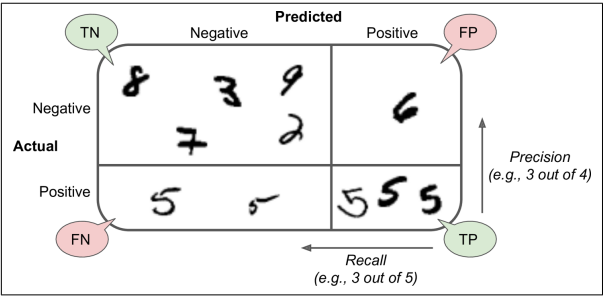
\includegraphics[width=0.60\linewidth,height=0.20\textheight]{Images/plot24}
\caption{Example from Digits Dataset}
\label{fig:multi}
\end{figure}

\item \textbf{Precision and Recall} : Ενώ ο πίνακας σύγχυσης περιέχει αρκετή πληροφορία δεν είναι μια μετρική.Μπορούμε λοπόν απο αυτόν να ορίσουυμε τις μετρικές:
$$precision = \frac{TP}{TP + FP} \ \ \  recall = \frac{TP}{TP + FN}$$
Η πρώτη δηλώνει την ακρίβεια των σωστών προβλέψεων , ενώ η δεύτερη τον λόγο των θετικών μετρήσεων όπου έχουν σωστά προβλεθεί απο τον ταξινομητή.Οι δύο αυτές μετρικές χρησιμοποιύνται μαζί καθώς η πρώτη μετρική απο μόνη της δεν μπορεί να παρέχει σημαντική πληροφορία.Αν θεωρήσουμε για παράδειγμα οτι έχουμε μια θετική πρόβλεωη και είναι σωστή τότε (precision = 1/1+0 =100\%), που βέβαια δεν εξασφαλίζει την ακρίβεια του ταξινομητή.

\item \textbf{F1 - score} : Πολλές φορές είναι βολικό να συνδυάζουμε τις μετρικές \textbf{precision and recall} σε μία μόνο μετρική η οποία ονομάζεται και harmonic mean των \textbf{precision and recall}.

$$F_1 = \frac{2}{\frac{1}{precision} + \frac{1}{recall}} = \frac{TP}{TP + \frac{FN + FP}{2}}$$


\item \textbf{The Rock Curve (Receiver Operating Characteristic)} : Είναι ένα πολύ γνωστό μέσο για την αξιολόγηση binary ταξινομητών.Σκοπός είναι να σχεδιάσουμε το true positive rate (TPR) προς το false positive rate (FPR).Όπου
$$TPR(T) = \int_T^{\infty} f_1(x)dx \ \ FPR(T) = \int_T^{\infty}f_0(x)dx$$
όπου T ένα όριο όπου αν $X>T \to "positive"$ αλλιώς "negative" , και η X $\sim f_1(x)$ αν ανήκει στην "positive" ενώ $\sim f_0(x)$ διαφορετικά.
\begin{figure}[H]
\centering
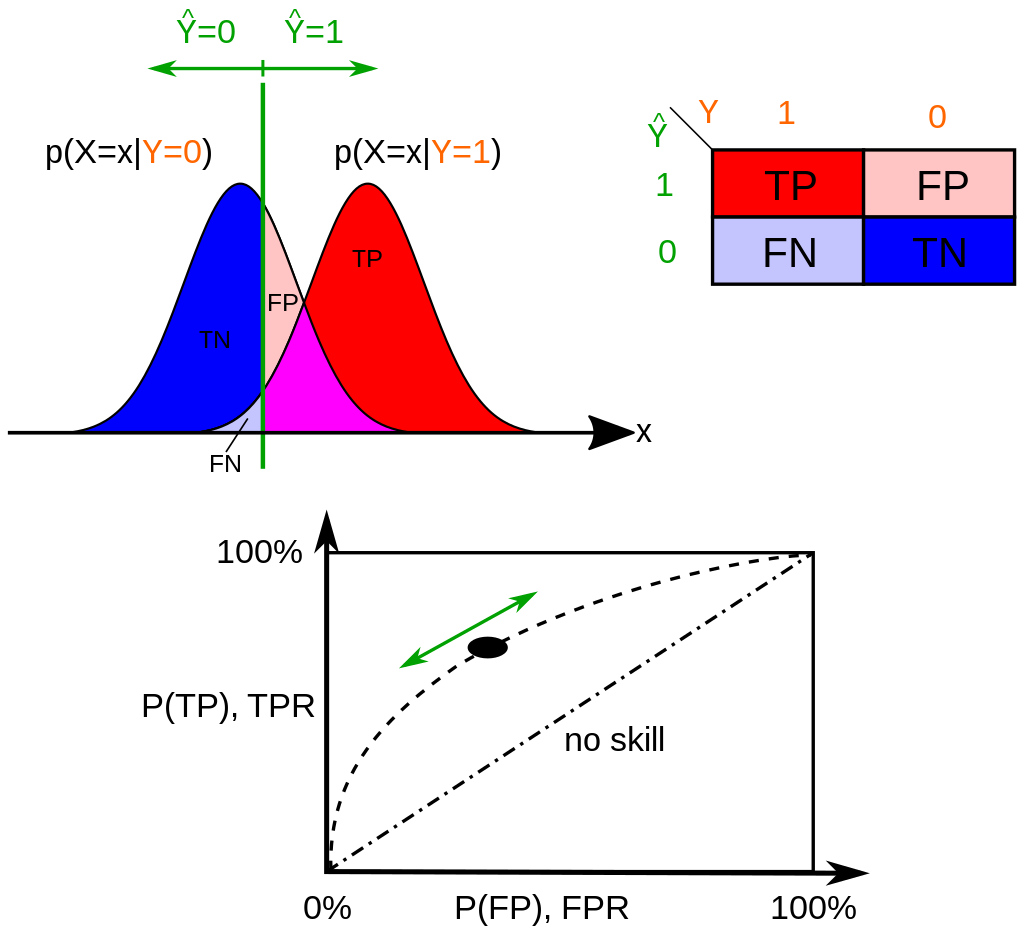
\includegraphics[width=0.50\linewidth,height=0.30\textheight]{Images/plot25}
\caption{ROC Curve}
\label{fig:multi}
\end{figure}

Η διακεκομένη αντιπροσωπεύει έναν ταξινομητή με κακή διακριτική ικανότητα  , όσο πιο μακρυά βρίσκεται η καμπύλη απο την ευθεία y =x τόσο καλυτερη η ακξριβεια του ταξινομητή.
\end{itemize}






\subsection{Feature Selection - Σημαντικότητα Παραμέτρων}
Για όσα έχουμε αναφέρει παραπάνω έχουμε ορι $\mathbb{X} = R^d$ δηλαδή κάθε παρατήρηση αντιπροσωπεύεται απο ένα διάνυσμα d μεταβλητών.Σκοπός μας είναι να δούμε αν μπορούμε να βρούμε ένα μοντέλο πρόβλεψηςε το οποίο αποτελείται απο  k <d μεταβλητές.Μια προσσεγγιση μελετήθηκε ήδη , χρησιμοποιώντας την μέθοδο PCA για να φτιάξουμε γραμμικούς συνδυανσμούτς των παραμέτρων μας και να καταλήξουμε σε ένα πρόβλημα μικρότερων διαστάσεων ( Feature Reduction).Βασικός λόγος που το θελουμε αυτό είναι το υπολογιστικό κόστος και όπως έχουμε αναφέρει το curse of Dimensionality.Ιδανικά θα θέλαμε να διαλέξουμε τις μεταβλητές k απο τις d που οδηγούν στο  "καλύτερο" μοντέλο , πράγμα που είναι υπλογιστικά δύκολο να δοκιμάσουμε όλους τους πιθανούς συνδυασμους.

\par \textbf{Backwards Elimination} :Στην εργασία μας θα χρησιμοποιήσουμε την μέθοδο Backwards Elimination για να διαλέξουμε τις πιο σημαντικές παραμέτρους στα μοντέλα που κατασκευάσαμε.Η μέθοδος αυτή ανήκει στην κλάση των \textbf{greedy} μεθόδων.Αρχικά ξεκινάμε με ένα σύνολο που περιέχει και τις d μεταβλητές του δειγματικού χώρου και σε κάθε βήμα αφαιρούμε μια μεταβλητή απο το σύνολο των μεταβλητών.Άρα θεωρώντας ένα σύνολο  I =\textbf{\{σύνολο μεταβλητών \} } , για κάθε $i \in I $ εφαρμόζουμε τον αλγόριθμο ταξινόμησης που έχουμε επιλέξει στο σύνολο $I/{i}$ και βλέπουμε ποιο μοντέλο με παραμέτρους απο το σύνολο $i \in I  $ έχει το μικρότερο ρίσκο (ή αντίστοιχα το μικρότερο σφάλμα).


\section{Αποτελέσματα}

\subsection{Least Squares LDA}



\subsection{Neural Network}


\subsection{Gradient Boosting Tree}





\end{document}
